\caption{Introdução}
\hspace{1.5cm}
Devido ao permanente estado de prontidão do Exército Brasileiro (EB), para atender as demandas da defesa nacional buscando a garantia da lei e da ordem, desenvolvimento nacional e o bem-estar social. Segundo \cite{operacao2017}, com o advento das mudanças na sociedade e a crescente utilização de  tecnologia nas operações militares, as guerras têm experimentado alterações significativas ao longo dos tempos. Com as atuais estruturas geopolíticas na história dos conflitos temos o aumento da importância dos fatos militares e não militares na busca da resolução das conflagrações, através de recentes capacidades.

\hspace{1.5cm}
Hoje mesmo com o advento tecnológico, nas suas diversas áreas, os conflitos convencionais, bem como as disputas de alta intensidade mantém suas condutas predominantes. Nos dias atuais o processo de decisão, sob uma ação de comando, deve ser realizada no momento adequado e com a maior brevidade possível. Neste contexto, é que os sistemas de Comando de Controle, em particular o Pacificador, tem a finalidade de ser uma fonte de apoio a decisão no conjunto das operações militares dentro de um plano ou ordem intentando cumprir uma atividade, tarefa, missão ou atribuição. 

\hspace{1.5cm}
O objetivo deste trabalho, é realizar uma análise estatística do uso do Pacificador, um sistema de comando e controle desenvolvido pelo Centro de Desenvolvimento de Sistemas e utilizado por várias Organizações Militares (OM) do EB. O escopo desta análise será discorrer sobre quais são os incidentes mais comuns, média de tempo de resolução dos incidentes ao longo dos anos, quantas e quais as operações o sistema já apoiou, quantos usuários já utilizaram, quais e quantos Centros de Operações foram criados.

\hspace{1.5cm}
A metodologia encontra-se dividida em três fases onde, na primeira fase, são coletados os dados do sistema, desde o momento de sua colocação em produção. Na segunda fase são analisados quais os dados poderão ser melhor comparados para que sejam geradas informações relevantes à pesquisa e, por fim, na terceira fase, são demonstradas as melhorias que o sistema trouxe à Força Terrestre e as possíveis melhorias que podem ser implementadas.

\hspace*{1.5cm}
A execução da abordagem metodológica, apresentada nesta seção, servirá como forma de trabalhar os conceitos estudados no referencial teórico, bem como responder às questões levantadas durante a apresentação do problema e justificativa da pesquisa, além de alcançar os objetivos do trabalho.



\section*{Comando e Controle}

\hspace{1.5cm}
Segundo \cite{undestanding2006}, a função Comando e Controle não é um fim em si mesmo, porém é meios para consegui criar valores (ex: o rastreamento de uma operação. Basicamente, C2 é sobre evidenciar esforços sobre determinados números de entidades, sendo elas Organizações ou pessoas, recursos, tais como informação gerando assim algumas tarefas, objetivos e metas. A definição de Comando e Controle é  incompleta e potencialmente inútil a menos que venha a prover medidas existentes. 

\hspace{1.5cm}
Mesmo o C2 sendo necessário ele não é a garantia do sucesso da operações. Este sucesso tem dependência de vários outros fatores, incluindo a disponibilidade dos meios apropriados, suas capacidades operacionais e além dos inimigos e outras adversidades do Teatro de Operação. O êxito de Comando e Controle não pode ser definido pelo o sucesso nas missões, levando em conta que missão é uma ação de comando.
% Talvez tenha que recuar pois copie todo o texto do EB20-MC-10.205
A definição de Comando e Controle encontrada no Manual EB20-MC-10.205 é:
\begin{quote}
 Constitui-se  no  exercício  da  autoridade  e  da  direção que um comandante tem sobre as forças sob o próprio comando, para o cumprimento da missão  designada.  Viabiliza  a  coordenação  entre  a  emissão  de  ordens  e  diretrizes  e  a  obtenção de informações sobre a evolução da situação e das ações desencadeadas. \cite{comandoecontrole2015}
\end{quote}
Esta concisa e limpa definição definição de C2 e suas terminologia estabelece o alicerce para o entendimento de como se dar o Comando e Controle. 

\hspace{1.5cm}
Conforme  \cite{comandoecontrole2015} \textit{Comando} representa a autoridade revestida de autoridade de comando dentro de uma ação/operação militar sobre os seus subordinados através de sua patente, em uma determinada tarefa. Já \textit{Controle}  é definido como a direção que o Comandante da a tua tropa e seu controle operacional. Independentemente de seu emprego ser colocado erroneamente, à medida que o comandante busca impor sua vontade no campo de batalha é imperativo que o controle porte-se em favor do comando. O triunfo em uma operação se dará pelo o efetivo adestramento em C2 por uma considerável tropa. Igualmente, uma força sem controle sobre os seus meios, pessoal e processos pode ser levada a derrota no teatro operacional. 

\hspace{1.5cm}
O Comando e Controle é coberto por três componentes  imprescindível e interdependentes, que são:
\begin{itemize}
    \item a autoridade, legalmente investida, de onde provém as decisões que materializam o exercício do comando, que influenciara no exercício de controle com o fluxo de informações.
    \item o processo decisório, baseado no arcabouço doutrinário, através da criação das ordens e determinado o caminho que deve seguir as informações até tua concretização.
    \item a estrutura, que inclui pessoal, instalações, equipamento e tecnologias que auxiliam na atividade de comando e controle.
\end{itemize}
Este componentes ajuda a estabelecer a relação de comando coma a intenção de mostrar ao comandante a dimensão em que sua autoridade é exercida, no processo hierárquico entre subordinados e superiores. No bloco subsequente conversaremos sobre a teoria de sistema de comando e controle. 

\section*{Sistema de Comando e Controle}
\hspace{1.5cm}
Segundo \cite{thesecommandandcontrol} a  principal missão do sistema de Comando e Controle (C2) é atender as necessidades dos comandantes. O sistema deve proporcionar aos comandantes tenham total uso de todos os recursos de forma efetiva e eficiente do emprego das forças militares por toda a extensão longitudinal dos conflitos. As três categorias de informação que é associada aos sistema de C2 são: status dos amigos, status dos inimigos e status do ambiente operacional. Todos os sistemas de C2 devem ser capaz de executar as seguintes funções básicas: coleta de dados; exibição dos processos; disseminação; e manter de dados a respeito da informação. O \cite{comandoecontrole2015} define sistema de Comando e Controle como: 
\begin{quote}
    Conjunto de instalações, equipamentos, comunicações, doutrina, procedimentos e pessoal essencial para o comandamento, em nível nacional, das crises e dos conflitos.
\end{quote}

\hspace{1.5cm}
A definição oficial em cinco básicos subconjuntos, para os sistema de C2: comunicações; pessoal;  doutrina; procedimento; instalações. A comunicações é o subsistema de entrada no sistema de C2, mas não é necessariamente o mais importante. Devido as  dificuldades dos Exércitos modernos na gerencia dos longos campos de batalha é requerido um capaz sistema de comunicações, para um efetivo e eficiente controle das forças. Com os avanços tecnológicos das comunicações a partir da 2ª Guerra Mundial, tem permitidos aos comandantes a manutenção de exercitar de C2 sobre as tropas. A ligação entre todos os componentes dos sistemas de C2 e os comandantes é realizados através das comunicações.

\hspace{1.5cm}
O pessoal é supostamente um significativo componente do sistema, haja vista que o homem é ao mesmo tempo a parte mais complexa e frágil. Em um sistema de C2 o homem fornece muitas entradas em todos os níveis. Estas entradas têm efeito direto no processo de decisão individual dos comandantes e nas suas percepções das informações  sobre os dados recebidos. O mal treinamento destes indivíduos ou sua afetação por ações de combate faz com que as informações contidas nos sistemas de C2 não sejam adequadamente úteis para os comandantes. Com o advento da tecnologia de inteligência artificial é um sistema de especialista utilizado para diminuir ou remover as baixas humanas no campo de batalha, porém não é um problema fácil de se resolver. A habilidade de reportar um problema por um subordinado, pode oferecer uma grande diferença na guerra, não sendo facilmente substituindo por um sistema automatizado.

\hspace{1.5cm}
Outro importante subconjunto do sistema de C2 são os equipamentos e instalações, somente aqueles que não fazem parte das comunicações e pessoal. Neles são incluídos os sensores, os computadores, os equipamentos de exibição, bem como, os locais onde será realizado a operação e manutenção dos equipamentos. Os computadores passaram a ser a principal peça dentro do processo de comando e controle. Devido a evolução tecnológica dos computadores dentro sistema de C2 passou a ser tão significativo que foi solicitado a mudança do termo C2 para C4 (acrescentado Comunicações e Computação). Computadores apresentam performance nas seguintes funções: sensores e comunicações de redes; correlação, filtragem e análise de informação sobre o inimigo; manutenção dos status e localização das forças amigas; viabilidade e estabelecimento dos planos desenvolvimento; e evolução dos planos de batalha e seus engajamentos. Os computadores aumentam a capacidade dos comandantes coletar e processar grande quantidade de dados, que facilita a sua capacidade de decisão. Mas, o comandante pode ficar saturado com a quantidade de informação, por isto é importante a utilização de um aplicativo com dados precisos, adequados, confiáveis e usualmente válido. A influência do homem tem impacto significativo no sistema de C2 na utilização da aplicação computacional. O grande desafio para comunidade de comando e controle é a operação de sistema de interoperável e no futuro a alta capacidades dos sistema de C2.

\hspace{1.5cm}
Dentro de um sistema de C2 está incluído todos os procedimentos usados para o planejamento, direção, coordenação e controle das forças na efetuação de uma determinada missão. Estes procedimentos são publicados pelo comandante que é o responsável pela performance das tarefas iniciadas e os pré-determinados padrões operacionais. Os modernos sistemas de C2 são complexos e constantemente cheio de tecnologia que são fundamental para função de comando e controle.

\hspace{1.5cm}
O entendimento da definição de Comando e Controle e os sistemas de C2, é a chave para entender as complexas estruturas organizacionais e operacionais deste sistema. O sistema Pacificador será descrito, como o sistema de C2 utilizados em grandes eventos e operações de GLO no nível estratégico. 

\section*{Sistema \textbf{\textit{Pacificador Web}}}

\hspace{1.5cm}
O Pacificador Web é um sistema de Comando e Controle (C2), membro da Família de aplicativos de Comando e Controle da Força Terrestre (FAC2FTer), utilizado pelo Ministério da Defesa (MD), pelas Forças Armadas e por diversas agências e órgãos de segurança nas operações de Garantia da Lei e da Ordem (GLO) e Grandes eventos. Foi amplamente empregado no período de 2012 e 2014, na Conferência das Nações Unidas para o Desenvolvimento Sustentável (Rio+20), Copa das Confederações, Jornada Mundial da Juventude e Copa do Mundo. Nestas operações o sistema mostrou-se extremamente útil para a manutenção da consciência situacional, tratamento de incidentes, sincronização de ações e apoio a decisão nos diversos escalões empregados, tendo sua utilização intensificada com a integração através de dispositivos móveis, tais como o Sistema Rádio Digital Troncalizado (SRDT) da Motorola, o sistema rádio Falcon III da Harris e sistemas de telefonia móvel com acesso à internet. Devido ao seu emprego bem sucedido nos grandes eventos, aṕos a Copa do Mundo surgiu a necessidade de utilização deste sistema em operações singulares da Força terrestre, tais como operações de Garantia da Lei e da Ordem (GLO) e de adestramento operacional dos comandos militares de área. 

\hspace{1.5cm}
O sistema Pacificador Móvel é um aplicativo desenvolvido para smartphones e tablets com sistema operacional Google Android sua finalidade é fazer que usuários de dispositivos móveis ligados a redes 3G/4G/5G possam inserir e consumir informações do Sistema Pacificador Web.
% \hspace{1.5cm}
\indent Tais informações consistem em:
\begin{itemize}
 \item posição geográfica em tempo real;
 \item relatos de situação;
 \item relatos de incidentes;e
 \item atualização de estado de ações;
\end{itemize}

% \emph{Detalhes sobre a operação do Pacificador Móvel devem ser consultados no seu manual.}

\hspace{1.5cm}
Convém salientar que as redes de telefonia móvel são gerenciadas por terceiros e portanto não é possível garantir o estabelecimento de conexão em locais com alta concentração de usuários como estádios e manifestações. A perda de conectividade nesta situação pode afetar o envio da posição geográfica em tempo real, o que não é defeito do aplicativo.

\hspace{1.5cm}
O Pacificador fundamenta-se no conceito de um Centro de Operações (COp), composto por operadores nas suas estruturas física e por agentes móveis. Os agentes móveis são integrantes do COp realizando tarefas diversas, como comboios, varreduras, segurança de instalações e escoltas. Eles têm consigo um telefone celular Android, com o sistema Pacificador Móvel instalado,  enviando sua localização ao Centro interligado, onde podem enviar relatos de situação, ocorrências e realizar ações a ele designadas na matriz. Outros agentes podem estar dotados de rádio, do sistema troncalizado, com suas localizações enviada através do Mups, Motorola, sendo que neste o Centro só terá visualização das localizações dos agentes no terreno.

\hspace{1.5cm}
Nas sede cada operador realiza o acompanhamento em tempo real dos relatos, ocorrências, localizações, e as realizações das ações de cada agente móvel, há muitas vezes uma tela de maiores dimensões ou um (ou mais) Videowall, com a finalidade de mostrar o cenário, com diversas localizações dos agentes, georreferenciado e em maior proporção destas informações. No Teatro de Operações pode existir mais de um COp, para cumprir a missão. O Pacificador Web compartilham continuamente, entre os Centros, informaçṍes relevantes que dão ao COp superior a visão e a capacidade de assumir a responsabilidade sobre as ações que deverão tomar os membros dos COps subordinados, além de delegar ações para os mesmos pela matriz de sincronização. Isto, gera a construção da Consciência Situacional Compartilhada, entre subordinados e decisor, no apoio da condução da operação.

\hspace{1.5cm}
Dentro do Sistema os agentes móveis foram divididos de acordo com o modo de operação, o qual caracteriza a função do agente naquele momento. As principais funções são: modo de agente de segurança, comboio, batedor, pontos de segurança, embarcações e escolta aérea. Os oficiais de ligação que geralmente são responsáveis por acompanhar as autoridades durante todos os deslocamentos e atividades oficiais, utiliza o modo comboio e agente de segurança respectivamente. O modo batedor é destinado aos batedores dos diversos sistemas de segurança que estiverem apoiando o Centro. As tropas realiza toda a segurança em diversos pontos específicos durante a GLO ou Grade evento usa o simbolo ponto de segurança. Já o modo de embarcação é utilizado para navios em geral e os helicópteros, basicamente dos BAvEx, é identificado pelo modo de escolta aérea. Todos os agentes móveis, sejam com rádios trocalizados ou smartphone, nos diversos modo de operação, transmite suas localizações que são replicada para os servidores, para que todos os COps, entre eles o COTer e Ministério da Defesa, alcance a consciência situacional. As transmissão das localizações pelos agentes em campo é realizada sem a intervenção do mesmo, bastando para isto está conectado aos uma dos servidores.

\hspace{1.5cm}
A implementação do Pacificador Web baseá-se nos conceitos técnicos, tais como: Consistência no COp, Consistência entre COps e Tolerância a Partição. A Consistência no COp se dar por sabemos que dentro de um mesmo Centro os diversos operadores buscam soluções para os mesmos conjuntos de problemas. Consequentemente, é relevante que a visão operacional seja comum para cada operador, bem como para o decisor, no cenário de arquitetura cliente-servidor. Na busca por uma Consciência Situacional Compartilhada entre os vários Centros de Operação, as informações de COps diferentes deve ser sincronizados. A Consistência entre COps se dará com o usuário acessando um mesmo servidor ou através de uma replicação de dados entre servidores. Com relação a Tolerância a partição o sistema deve ser to flexível a falhas de rede. O Pacificador está configurado em um pool de sítios em cidades diferentes para que cada Centro continue funcionando mesmo falta de contato entre alguns e quando a rede é recuperação os dados são sincronizados entre os servidores.

\hspace{1.5cm}
Implantação do Sistema Pacificador, que durante a Rio+20 era realizada nos 17 (dezessete) Centros de Operações na cidade do Rio de janeiro/RJ sofreu uma mudança significativa buscando atender a todos território Nacional. Na preparação para a Copas das Confederações no ano de 2013, foram realizado a implantação dos pool de servidores na cidade Brasília/DF e Rio de Janeiro. As cidades são contingências entre si, além de prover redundância em caso de falha, a existência destes dois pool é justificado pela necessidade de um atendimento nas constante na cidade do Rio de Janeiro. Os servidores localizados em Brasília/DF busca atender as demandas dos COps em todo o Brasil, pela EBNet.

\hspace{1.5cm}
Na próxima sessão será apresentado o Sistema Pacificador em números, através de algumas variáveis dentro da categoria CMilA.
\section*{Analise de Dados do Sistema Pacificador Web}
\hspace{1.5cm}
A construção de um modelo capaz de quantificar a utilização de Comando Militar, do Sistema de Comando e Controle, foi a realização de um estudo estatístico sobre as variáveis: centro de operação; agente; incidente; ação; e ponto de interesse,  colhidas na base de dados do sistema referente ao período de 2017 à out/2019, dos eventos e operações que aconteceram nestes período. Nesta análise exploratória, a hipótese era que o números das frequência das variáveis influencia a probabilidade de utilização da ferramenta para gerenciamento de Comando e Controle, pelos Comandante, da tropa nas diversas operações conjuntas. Basta ver, que é através das atuações dos agentes, determinadas pelos COps, mostra a utilização dos meios de comando e controle para criação de uma criação da Consciência Situacional de todo teatro de operação. 

\hspace{1.5cm}
Por conseguinte, o modelo proposto para quantificar a utilização do Sistema Pacificador, pelos Comandos Militares, será feita através da contagem de quantas observações se identificam nas categorias (frequências observadas) e mostra das percentagens de cada observação. Os valores obtidos servirão como base da análise deste estudo. 

\hspace{1.5cm}
Mais uma maneira de compreender a utilização dos sistema Pacificador e justificar teu uso é analisá-lo segundo o ciclo OODA\footnote{O ciclo OODA é um modelo que consigna um ciclo de decisão de quatro pontos que apoia uma decisão rápida e eficaz. Estes quatro pontos são: \textbf{Observar: }Recolher as informações atuais através de todas possíveis e disponíveis. \textbf{Orientar: }Analisar a informação recolhida e utilizá-la para atualizar a sua realidade. \textbf{Decidir: }Decidir o curso da ação. \textbf{Agir: }Implementar a sua decisão.}. As Ordens definem as quantidades de variáveis, que por sua vez influenciam na consciência situacional produzindo novas linhas de ação. Dessa maneira, o grau de utilização do programa é diretamente proporcional ao aumento quantitativo dos objetos por categoria analisada.

\hspace{1.5cm}
\textbf{Tabela \ref{QuantidadeCops}} É apresentado a distribuição de frequências do número de Centro de Operação (COps) numa amostra dos Comando Militar de Área do Exército Brasileiro. 

% Centro de Operação
\begin{table}[H]
\centering
\begin{tabular}{|c | c| c|} 
 \multicolumn{3}{c}{Centro de Operação por Comando Militar}\\ \hline
  Comando Militar & freq  & percentagem \\ [0.5ex] 
 \hline
 Comando Militar da Amazônia (CMA) & 35 & 7,17 \\ 
 \hline
 Comando Militar do Norte (CMN) & 48 & 9,84\\
 \hline
 Comando Militar do Nordeste (CMNE) &  90 & 18,44\\
 \hline
 Comando Militar do Centro-Oeste (CMO) & 42 & 8,61\\
 \hline
 Comando Militar do Planalto (CMP) &  65 & 13,32\\
 \hline
 Comando Militar do Sul (CMS) &  27 & 5,53\\
 \hline
 Comando Militar do Sudeste (CMSE) &  21 & 4,30\\
 \hline
 Comando Militar do Leste (CML) &  160 & 32,79\\ [1ex] 
 \hline
\end{tabular}
\caption{Quantidade de Centros de Operação por Comando Militar de Área}
\label{QuantidadeCops}
\end{table}

\hspace{1.5cm}
A representação gráfica da distribuição de frequência dos COps é dada pelo gráfico \ref{figuraCops}.
\begin{figure}[H]
        \centering
        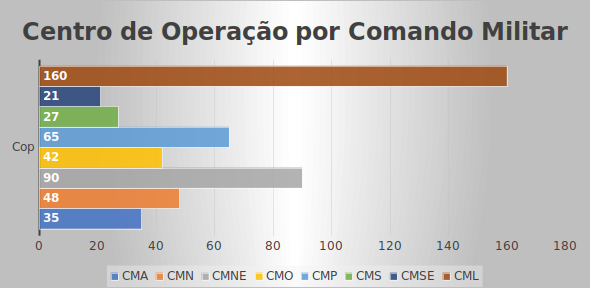
\includegraphics[width=1\textwidth]{imagens/qtde_cops.png}
        \caption{Gráfico de COps por Comandos Militar.}
        \label{figuraCops}
\end{figure}

\hspace{1.5cm}
\textbf{Tabela \ref{QuantidadeAgentes}} É apresentado a distribuição de frequências do número de Agente numa amostra dos Comando Militar de Área do Exército Brasileiro. 

% Agentes
\begin{table}[H]
\centering
\begin{tabular}{|c | c| c|} 
 \multicolumn{3}{c}{Agente por Comando Militar}\\ \hline
  Comando Militar & freq  & percentagem \\ [0.5ex] 
 \hline
 Comando Militar da Amazônia (CMA) &  1224 & 4,88\\ 
 \hline
 Comando Militar do Norte (CMN) &  1496 & 5,97\\
 \hline
 Comando Militar do Nordeste (CMNE) &  4350 & 17,36\\
 \hline
 Comando Militar do Centro-Oeste (CMO) &  336 & 1,34\\
 \hline
 Comando Militar do Planalto (CMP) &  1026 & 4,09\\
 \hline
 Comando Militar do Sul (CMS) &  350 & 1,40\\
 \hline
 Comando Militar do Sudeste (CMSE) &  2196 & 8,76\\
 \hline
 Comando Militar do Leste (CML) &  14082 & 56,19\\ [1ex] 
 \hline
\end{tabular}
\caption{Quantidade de Agentes por Comando Militar de Área}
\label{QuantidadeAgentes}
\end{table}

\hspace{1.5cm}
A representação gráfica da distribuição de frequência dos Agentes é dada pelo gráfico \ref{figuraAgentes}.
\begin{figure}[H]
        \centering
        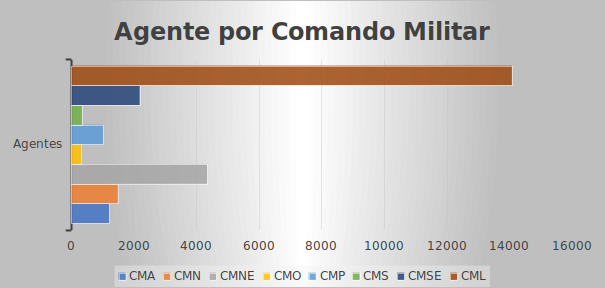
\includegraphics[width=1\textwidth]{imagens/qtde_agentes.png}
        \caption{Gráfico de Agentes por Comandos Militar.}
        \label{figuraAgentes}
\end{figure}

\hspace{1.5cm}
\textbf{Tabela \ref{QuantidadeIncidentes}} É apresentado a distribuição de frequências do número de Incidente numa amostra dos Comando Militar de Área do Exército Brasileiro. 
% Incidentes
\begin{table}[H]
\centering
\begin{tabular}{|c | c| c|} 
 \multicolumn{3}{c}{Incidente por Comando Militar}\\ \hline
  Comando Militar & freq   & percentagem \\ [0.5ex] 
 \hline
 Comando Militar da Amazônia (CMA) & 2280 & 21,80\\ 
 \hline
 Comando Militar do Norte (CMN) &  2301 & 22,00\\
 \hline
 Comando Militar do Nordeste (CMNE) &  3774 & 36,09\\
 \hline
 Comando Militar do Centro-Oeste (CMO) & 259 & 2,48\\
 \hline
 Comando Militar do Planalto (CMP) &  154 & 1,47\\
 \hline
 Comando Militar do Sul (CMS) &  203 & 1,94\\
 \hline
 Comando Militar do Sudeste (CMSE) &  79 & 0,76\\
 \hline
 Comando Militar do Leste (CML) &  1407 & 13,46\\ [1ex] 
 \hline
\end{tabular}
\caption{Quantidade de Incidentes por Comando Militar de Área}
\label{QuantidadeIncidentes}
\end{table}

\hspace{1.5cm}
A representação gráfica da distribuição de frequência dos Incidentes é dada pelo gráfico \ref{figuraIncidentes}.
\begin{figure}[H]
        \centering
        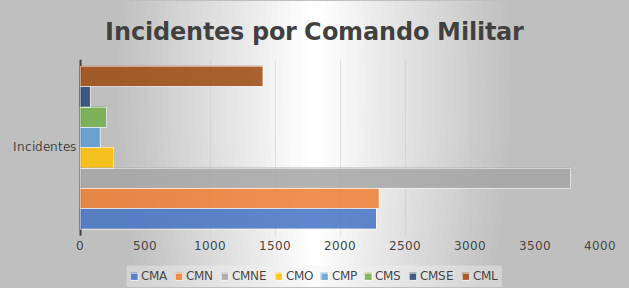
\includegraphics[width=1\textwidth]{imagens/qtde_incidentes.png}
        \caption{Gráfico de Incidentes por Comandos Militar.}
        \label{figuraIncidentes}
\end{figure}

\hspace{1.5cm}
\textbf{Tabela \ref{QuantidadeAcoes}} É apresentado a distribuição de frequências do número de Ação numa amostra dos Comando Militar de Área do Exército Brasileiro. 
% Ações
\begin{table}[H]
\centering
\begin{tabular}{|c | c| c|} 
 \multicolumn{3}{c}{Ação por Comando Militar}\\ \hline
  Comando Militar & freq   & percentagem \\ [0.5ex] 
 \hline
 Comando Militar da Amazônia (CMA) &  3193 & 22,22\\ 
 \hline
 Comando Militar do Norte (CMN) &  572 & 3,98\\
 \hline
 Comando Militar do Nordeste (CMNE) &  3009 & 20,94\\
 \hline
 Comando Militar do Centro-Oeste (CMO) &  3444 & 23,97\\
 \hline
 Comando Militar do Planalto (CMP) &  1031 & 7,18\\
 \hline
 Comando Militar do Sul (CMS) &  190 & 1,32\\
 \hline
 Comando Militar do Sudeste (CMSE) &  842 & 5,86\\
 \hline
 Comando Militar do Leste (CML) &  2087 & 14,53\\ [1ex] 
 \hline
\end{tabular}
\caption{Quantidade de Ações por Comando Militar de Área}
\label{QuantidadeAcoes}
\end{table}

\hspace{1.5cm}
A representação gráfica da distribuição de frequência dos Ações é dada pelo gráfico \ref{figuraAcoes}.
\begin{figure}[H]
        \centering
        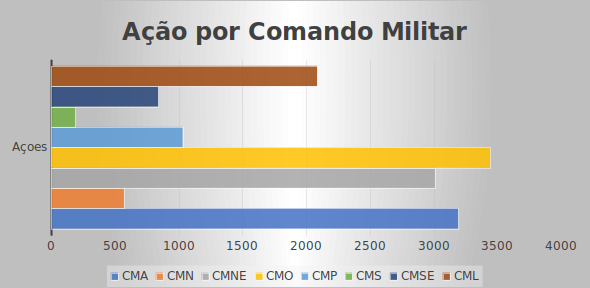
\includegraphics[width=1\textwidth]{imagens/qtde_acoes.png}
        \caption{Gráfico de Ações por Comandos Militar.}
        \label{figuraAcoes}
\end{figure}

\hspace{1.5cm}
\textbf{Tabela \ref{QuantidadeRelatos}} É apresentado a distribuição de frequências do número de Relato numa amostra dos Comando Militar de Área do Exército Brasileiro. 
% Relatos
\begin{table}[H]
\centering
\begin{tabular}{|c | c| c|} 
 \multicolumn{3}{c}{Relato por Comando Militar}\\ \hline
  Comando Militar & freq  & percentagem  \\ [0.5ex] 
 \hline
 Comando Militar da Amazônia (CMA) &  259 & 5,53\\ 
 \hline
 Comando Militar do Norte (CMN) &  371 & 7,93\\
 \hline
 Comando Militar do Nordeste (CMNE) &  1334 & 28,50\\
 \hline
 Comando Militar do Centro-Oeste (CMO) &  15 & 0,32\\
 \hline
 Comando Militar do Planalto (CMP) &  158 & 3,38\\
 \hline
 Comando Militar do Sul (CMS) &  611 & 13,06\\
 \hline
 Comando Militar do Sudeste (CMSE) &  1476 & 31,54\\
 \hline
 Comando Militar do Leste (CML) &  456 & 9,74\\ [1ex] 
 \hline
\end{tabular}
\caption{Quantidade de Relatos por Comando Militar de Área}
\label{QuantidadeRelatos}
\end{table}

\hspace{1.5cm}
A representação gráfica da distribuição de frequência dos Relatos é dada pelo gráfico \ref{figuraRelatos}.
\begin{figure}[H]
        \centering
        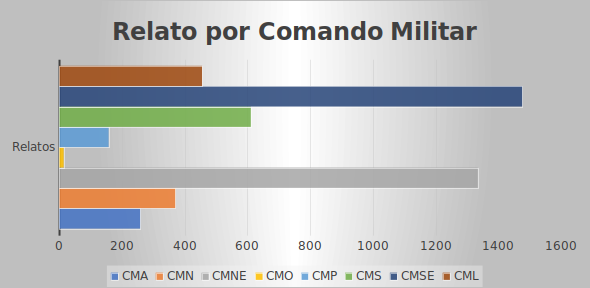
\includegraphics[width=1\textwidth]{imagens/qtde_relatos.png}
        \caption{Gráfico de Relatos por Comandos Militar.}
        \label{figuraRelatos}
\end{figure}

%\hspace{1.5cm}
%\textbf{Tabela \ref{QuantidadeKmls}} É apresentado a distribuição de frequências do número de Kml numa amostra dos Comando Militar de Área do Exército Brasileiro. 
% Kmls
% \begin{table}[H]
% \centering
% \begin{tabular}{|c | c| c|} 
%  \multicolumn{3}{c}{Kml por Comando Militar}\\ \hline
%   Comando Militar & freq  & percentagem  \\ [0.5ex] 
%  \hline
%  Comando Militar da Amazônia (CMA) &  40 & 11,17\\ 
%  \hline
%  Comando Militar do Norte (CMN) &  21 & 5,87\\
%  \hline
%  Comando Militar do Nordeste (CMNE) &  92 & 25,70\\
%  \hline
%  Comando Militar do Centro-Oeste (CMO) &  18 & 5,03\\
%  \hline
%  Comando Militar do Planalto (CMP) &  40 & 11,17\\
%  \hline
%  Comando Militar do Sul (CMS) &  4 & 1,12\\
%  \hline
%  Comando Militar do Sudeste (CMSE) &  14 & 3,91\\
%  \hline
%  Comando Militar do Leste (CML) &  129 & 36,03\\ [1ex] 
%  \hline
% \end{tabular}
% \caption{Quantidade de Kmls por Comando Militar de Área}
% \label{QuantidadeKmls}
% \end{table}

%\hspace{1.5cm}
%A representação gráfica da distribuição de frequência dos Kmls é dada pelo gráfico \ref{figuraKmls}
% \begin{figure}[H]
%         \centering
%         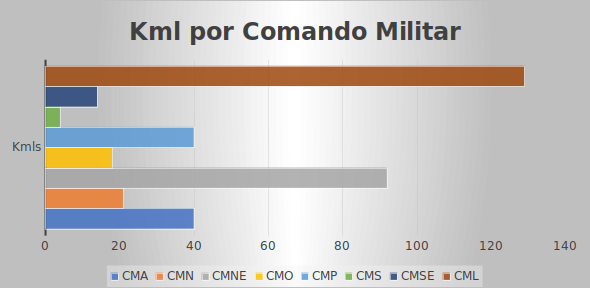
\includegraphics[width=1\textwidth]{imagens/qtde_kmls.png}
%         \caption{Gráfico de Kmls por Comandos Militar.}
%         \label{figuraKmls}
% \end{figure}

\hspace{1.5cm}
\textbf{Tabela \ref{QuantidadePois}} É apresentado a distribuição de frequências do número de Ponto de referência (POI) numa amostra dos Comando Militar de Área do Exército Brasileiro. 
% Pois
\begin{table}[H]
\centering
\begin{tabular}{|c | c| c|} 
 \multicolumn{3}{c}{Ponto de Interesse Operação por Comando Militar}\\ \hline
  Comando Militar & freq  & percentagem  \\ [0.5ex] 
 \hline
 Comando Militar da Amazônia (CMA) &  373 & \\ 
 \hline
 Comando Militar do Norte (CMN) &  61 & 3,44\\
 \hline
 Comando Militar do Nordeste (CMNE) &  357 & 20,16\\
 \hline
 Comando Militar do Centro-Oeste (CMO) &  14 & 0,79\\
 \hline
 Comando Militar do Planalto (CMP) &  55 & 3,11\\
 \hline
 Comando Militar do Sul (CMS) &  117 & 6,61\\
 \hline
 Comando Militar do Sudeste (CMSE) &  137 & 7,74\\
 \hline
 Comando Militar do Leste (CML) &  657 & 37,10\\ [1ex] 
 \hline
\end{tabular}
\caption{Quantidade de Ponto de interesse por Comando Militar de Área}
\label{QuantidadePois}
\end{table}

\hspace{1.5cm}
A representação gráfica da distribuição de frequência dos COps é dada pelo gráfico \ref{figuraPois}
\begin{figure}[H]
        \centering
        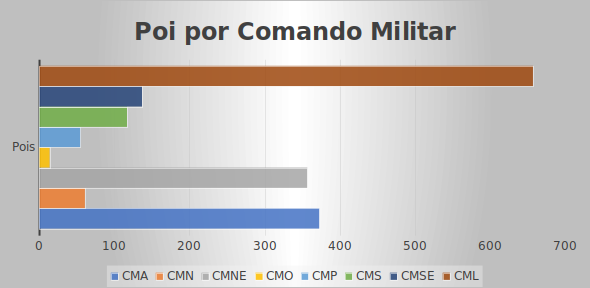
\includegraphics[width=1\textwidth]{imagens/qtde_pois.png}
        \caption{Gráfico de Pontos de interesse por Comandos Militar.}
        \label{figuraPois}
\end{figure}

\hspace{1.5cm}
Observamos nos resultados das figuras e gráficos percebemos que, através das frequências, das variáveis por categoria, a utilização do Sistema de Comando e Controle pelos os Comandos Militares de Área demostra o crescimento da ferramenta Pacificador como reforço aos Comandantes, nos diversos níveis, no controle dos elementos que compõe sua Força Tarefa durante uma determinado Grande evento, Operações e atividade de Garantia de Lei e Ordem.      

\section*{Conclusão}
\hspace{1.5cm}
Coloque aqui o texto\\